\chapter{Boundary and Initial Conditions}\label{sec:bcs}

%%%%%%%%%%%%%%%%%%%%%%%%%%%%%%%%%%%%%%%%%%%%%%%%%%%%%%%%%%%%%%%%%%%%%%%%%%%%%%%%
%%%%%%%%%%%%%%%%%%%%%%%%%%%%%%%%%%%%%%%%%%%%%%%%%%%%%%%%%%%%%%%%%%%%%%%%%%%%%%%%
\section{Background profiles}

The general form is given as a function of the coordinate $x_2$ according to
\begin{equation}
  f(x_2) = f_\text{ref}+\Delta f\, g(\xi) \;,\qquad
  \xi=\frac{x_2-x_{2,\text{ref}}}{\delta} \;,
\label{equ:profile}
\end{equation}
where the set of parameters $\{f_\text{ref},\,\Delta
f,\,x_{2,\text{ref}},\,\delta\}$ need to be provided, as well a the normalized
profile $g(\xi)$.

Possible forms are given in table~\ref{tab:profile} and
figure~\ref{fig:profile}. There are shear-like and jet-like profiles. In the
former case, the normalized profiles vary between $-1/2$ and $+1/2$, so that
equation~(\ref{equ:profile}) represents a variation of order $\Delta f$ around
the reference value $f_\text{ref}$ across a distance of order $\delta$ centered
around the position $x_{2,\text{ref}}$. The sign of $\delta$ can be used to
impose the symmetric form, if needed. The gradient thickness is defined by
\begin{equation}
  \delta_g =\frac{\Delta f}{|d f/d x_2|_\text{max}} =
  \delta\,\frac{1}{|d g/d \xi|_\text{max}} \;.
\label{equ:deltag}
\end{equation}
In the case in which the profile is used to define the mean velocity, this
thickness is known as vorticity thickness.  It is very often more convenient to
define the problem in terms of the gradient thickness instead of the thickness
parameter $\delta$. The reason to keep it in terms of $\delta$ in the code is
simply for compatibility with the previous versions.

\begin{SCfigure}
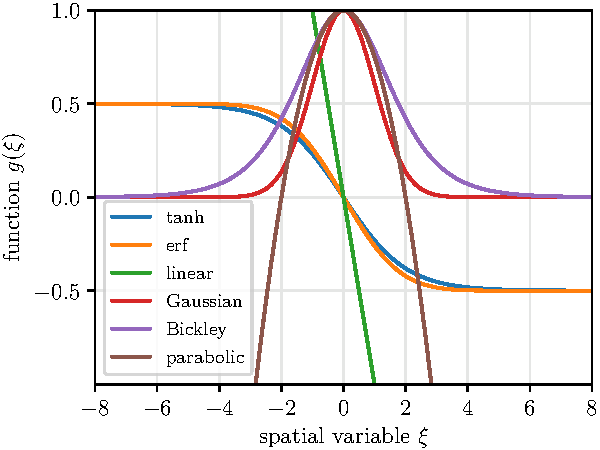
\includegraphics[clip,width=0.6\textwidth]{figs/profiles1}
\caption{Different normalized profiles used in equation~(\ref{equ:profile}). The
  black profiles provide shear-like backgrounds, the green lines provide
  jet-like backgrounds. These background profiles are used consistently for the
  boundary and initial conditions and aims at the study of different canonical
  flows, free and wall-bounded, shear- and buoyancy-driven.}\label{fig:profile}
\end{SCfigure}

The second group of profiles deliver a jet-like shape. In that case, $\Delta f$
provides the maximum difference with respect to the reference level
$f_\text{ref}$. The integral thickness is defined by
\begin{equation}
  \delta_i =\frac{1}{\Delta f}\int\! (f-f_\text{ref})\,\mathrm{d} x_2
  = \delta\int\! g(\xi)\mathrm{d}\,\xi \;.
\label{equ:deltai}
\end{equation}
According the implementation currently used, shown in table~\ref{tab:profile},
typical values are $2-3\delta$.

\begin{table}[!h]
\footnotesize
\renewcommand{\arraystretch}{1.2}
\centering
\rowcolors{1}{gray!25}{white}
\begin{tabular}{|l r r r p{0.4\textwidth}|}
%
\hline
\multicolumn{1}{>{\columncolor{gray!50}}c}{\bf Type} &
\multicolumn{1}{>{\columncolor{gray!50}}c}{\bf $\mathbf{g}(\boldsymbol{\xi})$} &
\multicolumn{1}{>{\columncolor{gray!50}}c}{\bf $\boldsymbol{\delta}_g/\boldsymbol{\delta}$ }&
\multicolumn{1}{>{\columncolor{gray!50}}c}{\bf $\boldsymbol{\delta}_i/\boldsymbol{\delta}$ }&
\multicolumn{1}{>{\columncolor{gray!50}}c}{\bf Notes}\\
\hline
Hyperbolic tangent  &  $(1/2)\tanh(-\xi/2)$ & $4$ & & Used in shear layer because it is the
reference profile commonly used in linear stability analysis. The parameter
$\delta$ is equal to the momentum thickness. Used because of available linear stability analysis.\\
Error function & $(1/2)\text{erf}(-\xi/2)$ & $2\sqrt{\pi}$ & & Used in diffusion dominated
problems because it is a solution of the diffusion equation.\\
Linear & $-\xi$ & 1 & & Varying $\Delta f$ along $\delta$.\\
Ekman & $1-\exp(-\xi)\cos(\xi)$& 1 & & Velocity component along geostrophic wind.\\
\rowcolor{gray!25}
  & $-\exp(-\xi)\sin(\xi)$&  & & Normal component. \\
\hline
Gaussian & $\exp(-\xi^2/2)$ & $1.65$ & $\sqrt{2\pi}$& Gaussian bell with standard deviation equal to $\delta$. \\
Bickley & $1/\cosh^2(\xi/2)$ & & $4$& Bell shape used in the linear stability of
jets. Used because of available linear stability analysis.\\
Parabolic & $(1+\xi/2)(1-\xi/2)$ & & $8/3$& Parabola crossing the
reference value at $x_{2,ref}\pm 2\delta$. Used for Poiseuille and channel
flows. The thickness $\delta_i$ is calculated using only the positive part of
the profile in the integral.\\
\hline
\end{tabular}
\caption{Different normalized profiles used in equation~(\ref{equ:profile}). The
  third column contains the gradient thickness $\delta_g$, defined by
  equation~(\ref{equ:deltag}), written explicitly as a function of the thickness
  parameter $\delta$. The fourth column contains the integral thickness
  $\delta_i$, defined by equation~(\ref{equ:deltai})}\label{tab:profile}
\end{table}

%%%%%%%%%%%%%%%%%%%%%%%%%%%%%%%%%%%%%%%%%%%%%%%%%%%%%%%%%%%%%%%%%%%%%%%%%%%%%%%%
%%%%%%%%%%%%%%%%%%%%%%%%%%%%%%%%%%%%%%%%%%%%%%%%%%%%%%%%%%%%%%%%%%%%%%%%%%%%%%%%
\section{Initial conditions}

There are several reasons to construct elaborated initial conditions beyond simply white random noise. For instance, to ascertain the duration of the initial transient before the flow enters into the fully developed turbulent regime; we can do that by varying the initial conditions and for that we need certain control of those initial conditions. We can also control certain aspects of that transient by using results from stability analysis and exciting or not certain modes; white noise simply excites all of them equally, and also that higher frequency content is dissipated much faster, which might render the energy amount that we use in the initialization misleading. In this respect, it maybe appropriate to say that the control of the duration of that transient is relatively difficult; on the other hand, the peak of turbulence intensities can be indeed controlled, if necessary e.g. because of resolution constraints. Third, it provides us with another tool to validate the code and algorithms, since we can compare results with analytical solutions.

The first step is to defined a mean background profile according to the previous section. For instance, a hyperbolic tangent profile for the mean streamwise velocity, $\bar{u}_1(x_2)$, while all other mean velocity components are set to zero.  The upper stream has a velocity $u_{1,ref}-\Delta u/2$ and the lower stream has a velocity $u_{1,ref}+\Delta u/2$ (see figure~\ref{fig:profile}). The mean density (or the mean temperature) can be similarly initialized, and a mean pressure is set to a uniform value $p_0$. The mean scalar can be similarly initialized.

In addition to the mean values, broadband fluctuations are used to accelerate the transition to turbulence. This is achieved by generating a random field on which is imposed an isotropic turbulence spectrum of one of the following forms:
\begin{equation}
  \begin{array}{lll}
    \text{uniform} &    E(f) = &1 \;,\\
    \text{quadratic} &  E(f) = &(f/f_0)^2 \exp[-2 (f/f_0)] \;,\\
    \text{quartic} &    E(f) = &(f/f_0)^4 \exp[-2 (f/f_0)^2] \;,\\
    \text{Gaussian} &   E(f) = & \exp[-(1/2)(f/f_0-1)^2/(\sigma/f_0)^2] \;,
  \end{array}
  \label{equ:spectra}
\end{equation}
where $f$ is the spatial frequency and $f_0$ is the peak spatial frequency. The extent of the turbulence is limited in the cross-stream direction by an exponential decay over a specified thickness of the order of the initial shear layer thickness. The solenoidal constraint is imposed on this random turbulent field. Such quasi-incompressible fluctuations minimize compressibility transients \cite{Erlebacher:1990}. The pressure fluctuations are obtained from the Poisson equation for incompressible flow.

\begin{SCfigure}
  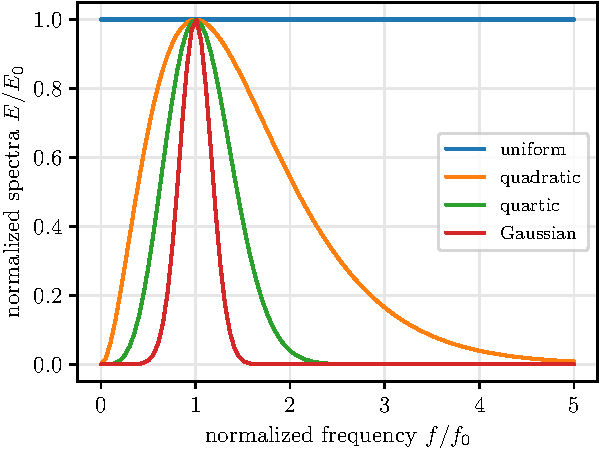
\includegraphics[clip,width=0.6\textwidth]{figs/spectra}
  \caption{Different power spectral densities available as initial conditions, equation~(\ref{equ:spectra}). Normalized such that all of them have equal integral. The Gaussian profile is plotted for the case $\sigma/f_0=1/6$ typically used in the simulations.}
  \label{fig:eq-spc}
\end{SCfigure}

%%%%%%%%%%%%%%%%%%%%%%%%%%%%%%%%%%%%%%%%%%%%%%%%%%%%%%%%%%%%%%%%%%%%%%%%%%%%%%%%
%%%%%%%%%%%%%%%%%%%%%%%%%%%%%%%%%%%%%%%%%%%%%%%%%%%%%%%%%%%%%%%%%%%%%%%%%%%%%%%%
\section{Boundary conditions}

\subsection{Compressible formulation}

For non-periodic directions, the treatment of the boundary conditions in the
periodic formulation is done in characteristic form
\citep{Thompson:1987,Thompson:1990,Lodato:2008}.

\subsection{Incompressible formulation}

To be developed.

\subsection{Buffer zone}\label{sec:buffer}

Buffer or sponge zones can be considered at the beginning and at the end of the
directions $Ox$ and $Oy$. These are simply defined by specifying the number of
points over which they extend. We can consider a filter or a relaxation form.

Regarding the relaxation form, we simply add
\begin{equation}
\left(\frac{\delta \mathbf{q}}{\delta t}\right)_b=-\tau_q^{-1}(\mathbf{q}-\mathbf{q}_0)
\;,\qquad
\left(\frac{\delta \mathbf{s}}{\delta t}\right)_b=-\tau_s^{-1}(\mathbf{s}-\mathbf{s}_0)
\end{equation}
to the right-hand sides of the transport equations \citep{Hu:1996b}.  The
relaxation times $\tau(\mathbf{x})$ are defined in terms of a power function as
\begin{equation}
  \tau_q^{-1}=\alpha_1(n-n_0)^{\alpha_2} \;,\qquad
  \tau_s^{-1}=\beta_1(n-n_0)^{\beta_2}
\end{equation}
where $n$ is the coordinate normal to the corresponding boundary and $n_0$ the
coordinate where the buffer region begins. The coefficients $\alpha_i$ and
$\beta_i$ need to be provided, the exponents being preferably larger or equal
than 2 so than the pressure equation has a continuous right-hand side.  The
reference fields $\mathbf{q}_0(\mathbf{x})$ and $\mathbf{s}_0(\mathbf{x})$ also
need to be provided and it can be any general field. Normally, a reference field
is created at some moment in the simulation (generally the initial time) as an
average of the corresponding region in the flow and scalar fields.
